% Options for packages loaded elsewhere
\PassOptionsToPackage{unicode}{hyperref}
\PassOptionsToPackage{hyphens}{url}
%
\documentclass[
]{article}
\usepackage{amsmath,amssymb}
\usepackage{iftex}
\ifPDFTeX
  \usepackage[T1]{fontenc}
  \usepackage[utf8]{inputenc}
  \usepackage{textcomp} % provide euro and other symbols
\else % if luatex or xetex
  \usepackage{unicode-math} % this also loads fontspec
  \defaultfontfeatures{Scale=MatchLowercase}
  \defaultfontfeatures[\rmfamily]{Ligatures=TeX,Scale=1}
\fi
\usepackage{lmodern}
\ifPDFTeX\else
  % xetex/luatex font selection
\fi
% Use upquote if available, for straight quotes in verbatim environments
\IfFileExists{upquote.sty}{\usepackage{upquote}}{}
\IfFileExists{microtype.sty}{% use microtype if available
  \usepackage[]{microtype}
  \UseMicrotypeSet[protrusion]{basicmath} % disable protrusion for tt fonts
}{}
\makeatletter
\@ifundefined{KOMAClassName}{% if non-KOMA class
  \IfFileExists{parskip.sty}{%
    \usepackage{parskip}
  }{% else
    \setlength{\parindent}{0pt}
    \setlength{\parskip}{6pt plus 2pt minus 1pt}}
}{% if KOMA class
  \KOMAoptions{parskip=half}}
\makeatother
\usepackage{xcolor}
\usepackage[margin=1in]{geometry}
\usepackage{graphicx}
\makeatletter
\def\maxwidth{\ifdim\Gin@nat@width>\linewidth\linewidth\else\Gin@nat@width\fi}
\def\maxheight{\ifdim\Gin@nat@height>\textheight\textheight\else\Gin@nat@height\fi}
\makeatother
% Scale images if necessary, so that they will not overflow the page
% margins by default, and it is still possible to overwrite the defaults
% using explicit options in \includegraphics[width, height, ...]{}
\setkeys{Gin}{width=\maxwidth,height=\maxheight,keepaspectratio}
% Set default figure placement to htbp
\makeatletter
\def\fps@figure{htbp}
\makeatother
\setlength{\emergencystretch}{3em} % prevent overfull lines
\providecommand{\tightlist}{%
  \setlength{\itemsep}{0pt}\setlength{\parskip}{0pt}}
\setcounter{secnumdepth}{-\maxdimen} % remove section numbering
\ifLuaTeX
  \usepackage{selnolig}  % disable illegal ligatures
\fi
\usepackage{bookmark}
\IfFileExists{xurl.sty}{\usepackage{xurl}}{} % add URL line breaks if available
\urlstyle{same}
\hypersetup{
  pdftitle={Assignment 1},
  hidelinks,
  pdfcreator={LaTeX via pandoc}}

\title{Assignment 1}
\author{}
\date{\vspace{-2.5em}2025-02-21}

\begin{document}
\maketitle

\paragraph{Group members: Keerthi (s243933), Katarina (s243906), Hubert
(s243896), German
(s243660)}\label{group-members-keerthi-s243933-katarina-s243906-hubert-s243896-german-s243660}

\subsection{1 Plot data}\label{plot-data}

\subsubsection{1.1.}\label{section}

\begin{figure}

{\centering \includegraphics[width=0.7\linewidth]{plots/dtrain_plot} 

}

\caption{The plot of observations.}\label{fig:unnamed-chunk-1}
\end{figure}

\subsubsection{1.2.}\label{section-1}

There seems to be a general positive trend of number of vehicles in
Denmark over the years. However, there is also a seasonal pattern within
each year where it increases for approximately the first half of a year
and then decreases. We also noticed that there is a jump at the start of
2021, and also after that the trend seems to have gotten flatter but the
seasonal pattern still exists.

\subsubsection{2 Linear trend model}\label{linear-trend-model}

\paragraph{2.1}\label{section-2}

{[}todo{]} {[}for each member{]} \[
y = \begin{bmatrix}
2.930 \\
2.934 \\
2.941
\end{bmatrix},
\quad
X = \begin{bmatrix}
1 & 2018.000 \\
1 & 2018.083 \\
1 & 2018.167
\end{bmatrix}
\]

\subsubsection{2.2}\label{section-3}

\begin{table}[h]
\centering
\begin{tabular}{|l|c|c|}
\hline
\textbf{Parameter} & \textbf{Estimate} ($\hat{\theta}$) & \textbf{Standard Error} ($\hat{\sigma}_{\hat{\theta}}$) \\
\hline
$\hat{\theta}_1$ & -110.36 & 3.59 \\
\hline
$\hat{\theta}_2$ & 0.056 & 0.0018 \\
\hline
\end{tabular}
\caption{Parameter Estimates and Standard Errors}
\label{tab:parameters}
\end{table}

\begin{figure}

{\centering \includegraphics[width=0.7\linewidth]{plots/estimated_mean} 

}

\caption{Observations and OLS Estimated Mean}\label{fig:unnamed-chunk-2}
\end{figure}

\subsubsection{2.3}\label{section-4}

The forecast results are presented in Table \ref{tab:forecast-results}.

\begin{table}[htbp]
\centering
\caption{Forecast Results}
\label{tab:forecast-results}
\begin{tabular}{cccc}
\hline
& fit & lwr & upr \\
\hline
73 & 3.281154 & 3.227579 & 3.334728 \\
74 & 3.285832 & 3.232198 & 3.339467 \\
75 & 3.290511 & 3.236815 & 3.344208 \\
76 & 3.295190 & 3.241430 & 3.348950 \\
77 & 3.299869 & 3.246044 & 3.353693 \\
78 & 3.304547 & 3.250656 & 3.358439 \\
79 & 3.309226 & 3.255267 & 3.363185 \\
80 & 3.313905 & 3.259876 & 3.367934 \\
81 & 3.318583 & 3.264483 & 3.372683 \\
82 & 3.323262 & 3.269090 & 3.377435 \\
83 & 3.327941 & 3.273694 & 3.382188 \\
84 & 3.332620 & 3.278297 & 3.386942 \\
\hline
\end{tabular}
\end{table}

\subsubsection{2.4}\label{section-5}

The plot is represented in Figure \ref{fig:fig-total-plot}.

\begin{figure}

{\centering \includegraphics[width=0.7\linewidth]{plots/total_plot} 

}

\caption{\label{fig:fig-total-plot}Fitted model together with the training data and the forecasted values.}\label{fig:unnamed-chunk-3}
\end{figure}

\subsubsection{2.5}\label{section-6}

The forecast appears to be limited as it overshoots the actual values
with a slope that doesn't align with the patterns, especially during the
test period. The inaccuracy is further demonstrated by most forecasted
values falling outside the prediction interval. All in all, this is a
basic forecast, following the general trend of the data, but not
seasonal shifts.

\subsubsection{2.6}\label{section-7}

The residuals show confusing patterns, staying close to the reference
line only in the middle while significantly deviating at both the
beginning and end of the plot. The model assumptions seem to be violated
as the errors aren't properly distributed around zero, with negative
residuals indicating the forecast systematically overshoots actual
values. This systematic error pattern suggests fundamental issues with
the model specification rather than random noise, confirming the model
assumptions are not fulfilled.

\subsection{3 WLS - local linear trend
model}\label{wls---local-linear-trend-model}

\subsubsection{3.1}\label{section-8}

The variance-covariance matrix for the local model consists of the
inverse of observation weights in the diagonal and zeros otherwise.
\(N\) is equal to the number of observation, which is equal to \(72\).
\[
\Sigma_{WLS} = 
\begin{pmatrix}
\frac{1}{\lambda^{N-1}} & 0 & \cdots & 0 \\
0 & \frac{1}{\lambda^{N-2}} & \cdots & 0 \\
\vdots & \vdots & \ddots & \vdots \\
0 & 0 & \cdots & \frac{1}{\lambda^{0}}
\end{pmatrix}
\] Conversely, the variance-covariance matrix for the global model
contains \(1\) in the diagonal and zeros otherwise. \[
\Sigma_{OLS}= 
\begin{pmatrix}
1 & 0 & \cdots & 0 \\
0 & 1 & \cdots & 0 \\
\vdots & \vdots & \ddots & \vdots \\
0 & 0 & \cdots & 1
\end{pmatrix}
\]

\subsubsection{3.2}\label{section-9}

The highest weight is for the latest time point and it is equal to
\(\lambda^0 = 1\). The further in the past an observation point is, the
more does its weight decrease. The weight distribution is visualized in
Figure \ref{fig:weights}.

\begin{figure}

{\centering \includegraphics[width=0.7\linewidth]{plots/weights_wls} 

}

\caption{\label{fig:weights}The weights of each observation in the train dataset.}\label{fig:unnamed-chunk-4}
\end{figure}

\subsubsection{3.3}\label{section-10}

The sum of weights for the local model is
\(\sum_{n=1}^{N} \lambda^{n-1} = 9.994925\). The sum of weights for the
global model is equal to the number of observations, \(72\).

\subsubsection{3.4}\label{section-11}

According to the local model with \(\lambda = 0.9\), the parameters are
equal to \(\theta_1=-52.4828617\) and \(\theta_2=0.0275299\).

\subsubsection{3.5}\label{section-12}

The WLS model prioritizes recent data points, creating a more gradual
slope that adapts to current trends. While OLS treats all data equally
and provides a generalized fit, WLS gives higher weight to recent
observations. We would choose WLS when new predictions are crucial, and
OLS when analyzing from a long-term perspective.

\begin{figure}

{\centering \includegraphics[width=0.7\linewidth]{plots/ols_wls_prediction} 

}

\caption{The observations as well as the predictions for the OLS \& WLS models, including prediction intervals.}\label{fig:unnamed-chunk-5}
\end{figure}

\subsection{\texorpdfstring{4 Recursive estimation and optimization of
\(\lambda\)}{4 Recursive estimation and optimization of \textbackslash lambda}}\label{recursive-estimation-and-optimization-of-lambda}

\subsubsection{4.1}\label{section-13}

{[}todo{]}

\subsubsection{4.2}\label{section-14}

{[}todo{]}

\subsubsection{4.3}\label{section-15}

{[}todo{]}

\subsubsection{4.4}\label{section-16}

{[}todo{]}

\subsubsection{4.5}\label{section-17}

\begin{figure}

{\centering 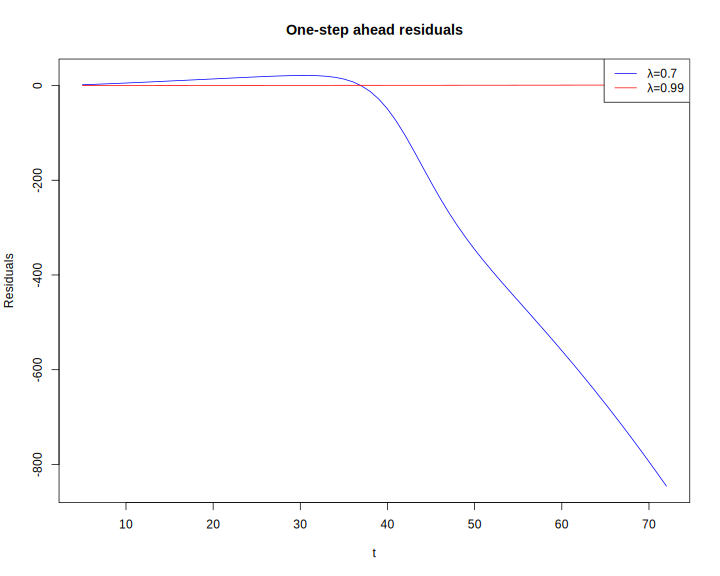
\includegraphics[width=0.5\linewidth]{plots/one_step_ahead_pred} 

}

\end{figure}

The plot above shows the one-step-ahead residuals for \(\lambda = 0.7\)
in blue and \(\lambda = 0.99\) in red. The residuals represent the
difference between predicted and actual values at each time step. For
\(\lambda = 0.99\), the residuals are stable, showing that the model is
more resistant to any recent fluctuations because of the higher weight
given to past observations. In contrast, for \(\lambda = 0.7\), the
residuals diverge a lot more, suggesting that the model reacts stronger
to recent data. This clearly shows how the choice of \(\lambda\) affects
the stability and adaptability of the recursive estimation process.

\subsubsection{4.6}\label{section-18}

\begin{figure}

{\centering \includegraphics[width=0.5\linewidth]{plots/rmse_lambda} 

}

\end{figure}

The relationship between the forgetting factor \(\lambda\) and the Root
Mean Square Error (RMSE) across different forecast horizons
(\(k = 1, \dots, 12\)) is shown. A clear trend can be noticed where RMSE
decreases as \(\lambda\) approaches \(1\), meaning that a higher
\(\lambda\) results in lower prediction errors. However, for lower
values of \(\lambda\), the RMSE is much higher, which could mean that
too much ``forgetting'' doesn't gives optimal predictions. These results
would then suggest that the optimal choice of \(\lambda\) lies within
the range of 0.8 to 0.99, where RMSE is minimized. Moreover, since the
RMSE patterns are the same across all horizons, I would use a single
optimal \(\lambda\) rather than letting it depend on the horizon.

\subsubsection{4.7}\label{section-19}

{[}todo{]}

\subsubsection{4.8}\label{section-20}

Time adaptive models are very useful for tracking changes of a dynamic
system. However, they also come with a set of challenges that should be
carefully considered or managed. One concern is to balance adaptation
speed with stability. If \(\lambda\) is too small, the model relies on
recent data which makes is very sensitive to fluctuations and noise. On
the other hand, if \(\lambda\) is too high, our older data will have a
stronger imact which then makes the model unresponsive to new trends. In
other words, our model overfits or underfits and selecting the right
\(\lambda\) value is crucial for good generalization.

Time dependent data also introduces autocorrelation which makes
cross-validation less effective. This is because splitting data randomly
leads to data leakage where future data influences past predictions.
Instead, time dependent data requires sequential train-test splits such
as rolling windows that make for a more realistic evaluation of the
model performance.

Recursive estimation helps with challenges with test sets for time
dependent data by allowing the model to update its predictions
recursively as new data comes. So, instead of relying on a fixed set,
the model refines its parameters and learns any new trends.

An alternative technique for adaptive estimation is the long short-term
memory network that is designed to capture temporal dependencies and
adapt over time.

\end{document}
